\documentclass[11pt]{article}
\usepackage[margin=1in]{geometry}
\usepackage{amsmath,amssymb,amsthm}
\usepackage{booktabs}
\usepackage{graphicx}
\usepackage{xcolor}
\usepackage{tikz}
\usetikzlibrary{arrows.meta,positioning,calc}
\usepackage[hidelinks]{hyperref}
\usepackage{caption}
\usepackage{parskip}
\usepackage{float}
\usepackage{tabularx}
\usepackage{multirow}
\usepackage{listings}
\lstset{language=Python, basicstyle=\ttfamily\scriptsize, columns=fullflexible, keepspaces=true,
  frame=single, rulecolor=\color{black!25}, backgroundcolor=\color{black!3}, commentstyle=\color{ink2}\itshape,
  keywordstyle=\color{cbase}\bfseries, stringstyle=\color{cfive}, showstringspaces=false, breaklines=true,
  breakatwhitespace=true, postbreak=\mbox{\textcolor{ink2}{$\hookrightarrow$}\space}, aboveskip=4pt, belowskip=6pt,
  xleftmargin=2pt, xrightmargin=2pt, upquote=true}

% auto-generated by train/make_variant_report.py
\newcommand{\BaseSteps}{4768}
\newcommand{\BaseTok}{2.50B}
\newcommand{\BaseAtA}{5.741}
\newcommand{\BaseAtB}{4.733}
\newcommand{\BaseAtC}{3.871}
\newcommand{\BaseAtD}{3.465}
\newcommand{\BaseAtE}{3.312}
\newcommand{\BaseTwenty}{3.312}
\newcommand{\BaseFour}{3.191}
\newcommand{\BaseDelta}{+0.000}
\newcommand{\BaseInitRank}{0.717}
\newcommand{\BaseInitCos}{0.487}
\newcommand{\BaseTrRank}{0.877}
\newcommand{\BaseKL}{4.356}
\newcommand{\OneSteps}{3951}
\newcommand{\OneTok}{2.07B}
\newcommand{\OneAtA}{7.665}
\newcommand{\OneAtB}{7.642}
\newcommand{\OneAtC}{7.649}
\newcommand{\OneAtD}{7.632}
\newcommand{\OneAtE}{7.632}
\newcommand{\OneTwenty}{7.652}
\newcommand{\OneFour}{7.632}
\newcommand{\OneDelta}{+4.340}
\newcommand{\OneInitRank}{0.029}
\newcommand{\OneInitCos}{0.999}
\newcommand{\OneTrRank}{0.002}
\newcommand{\OneKL}{0.005}
\newcommand{\TwoSteps}{3741}
\newcommand{\TwoTok}{1.96B}
\newcommand{\TwoAtA}{7.665}
\newcommand{\TwoAtB}{7.642}
\newcommand{\TwoAtC}{7.647}
\newcommand{\TwoAtD}{7.632}
\newcommand{\TwoAtE}{7.631}
\newcommand{\TwoTwenty}{7.652}
\newcommand{\TwoFour}{7.631}
\newcommand{\TwoDelta}{+4.339}
\newcommand{\TwoInitRank}{0.030}
\newcommand{\TwoInitCos}{0.999}
\newcommand{\TwoTrRank}{0.000}
\newcommand{\TwoKL}{0.004}
\newcommand{\ThreeSteps}{4768}
\newcommand{\ThreeTok}{2.50B}
\newcommand{\ThreeAtA}{5.793}
\newcommand{\ThreeAtB}{4.755}
\newcommand{\ThreeAtC}{3.875}
\newcommand{\ThreeAtD}{3.478}
\newcommand{\ThreeAtE}{3.323}
\newcommand{\ThreeTwenty}{3.324}
\newcommand{\ThreeFour}{3.202}
\newcommand{\ThreeDelta}{+0.011}
\newcommand{\ThreeInitRank}{0.696}
\newcommand{\ThreeInitCos}{0.515}
\newcommand{\ThreeTrRank}{0.878}
\newcommand{\ThreeKL}{4.329}
\newcommand{\FourSteps}{4768}
\newcommand{\FourTok}{2.50B}
\newcommand{\FourAtA}{7.665}
\newcommand{\FourAtB}{7.614}
\newcommand{\FourAtC}{7.640}
\newcommand{\FourAtD}{7.631}
\newcommand{\FourAtE}{7.633}
\newcommand{\FourTwenty}{7.646}
\newcommand{\FourFour}{7.623}
\newcommand{\FourDelta}{+4.334}
\newcommand{\FourInitRank}{0.030}
\newcommand{\FourInitCos}{0.999}
\newcommand{\FourTrRank}{0.001}
\newcommand{\FourKL}{0.007}
\newcommand{\FiveSteps}{4768}
\newcommand{\FiveTok}{2.50B}
\newcommand{\FiveAtA}{5.921}
\newcommand{\FiveAtB}{5.015}
\newcommand{\FiveAtC}{4.013}
\newcommand{\FiveAtD}{3.534}
\newcommand{\FiveAtE}{3.364}
\newcommand{\FiveTwenty}{3.355}
\newcommand{\FiveFour}{3.234}
\newcommand{\FiveDelta}{+0.043}
\newcommand{\FiveInitRank}{0.327}
\newcommand{\FiveInitCos}{0.894}
\newcommand{\FiveTrRank}{0.872}
\newcommand{\FiveKL}{4.295}
\newcommand{\RefTwenty}{3.295}
\newcommand{\RefFour}{3.204}
\newcommand{\UniTwenty}{7.649}
\newcommand{\UniFour}{7.631}


\newcommand{\code}[1]{\texttt{#1}}
\definecolor{ink2}{HTML}{52514e}
\definecolor{cbase}{HTML}{2a78d6}
\definecolor{cone}{HTML}{eb6834}
\definecolor{ctwo}{HTML}{1baf7a}
\definecolor{cthree}{HTML}{c98500}
\definecolor{cfour}{HTML}{d55181}
\definecolor{cfive}{HTML}{008300}
\definecolor{okfill}{HTML}{e8f1fb}
\definecolor{badfill}{HTML}{fdecea}
\definecolor{midfill}{HTML}{e9f5e9}
\newtheorem{prop}{Proposition}
\newcommand{\cat}{\mathrm{Concat}_h}

\title{Attention-Residual Variants of GPT-2 124M:\\Structure, Performance, and Why Some Collapse}
\author{Experiment log, branch \code{attention-experiments}}
\date{2026-10-16}

\begin{document}
\maketitle

\section*{Summary}
Five modifications of GPT-2's attention sublayer (approach\_1 to approach\_5) and the original GPT-2
(\emph{baseline}) were each trained from scratch for a Chinchilla-optimal budget: 2.5B FineWeb-Edu tokens,
same data order, same hyperparameters, same seed. All of them feed the raw residual stream $X$ into
attention in some form. They differ in how the token's own state is carried to the next layer.

\begin{figure}[H]
\centering
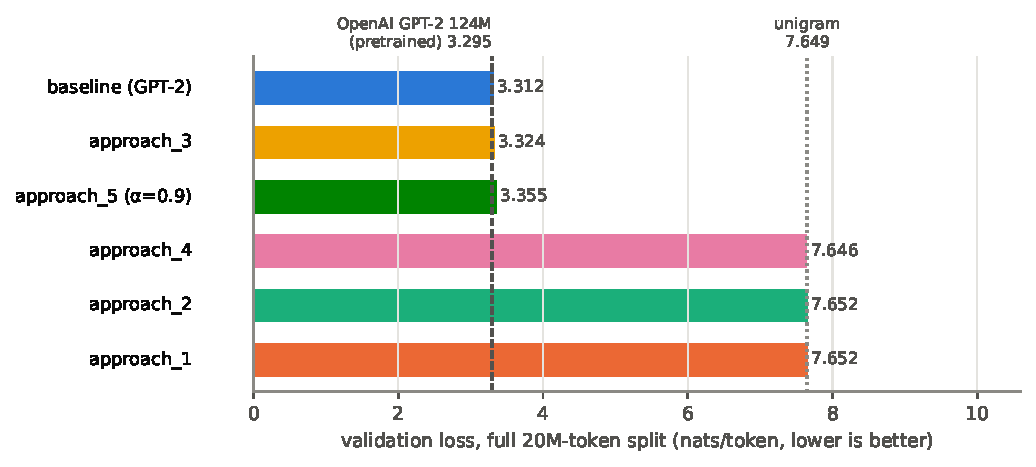
\includegraphics[width=0.92\linewidth]{figures/fig_final_loss.pdf}
\caption{Final validation loss on the full 20M-token split. approach\_1/2 are scored at their last checkpoint
(step 3000). All the others, approach\_4 included, are scored at their final checkpoint (step 4768).}
\label{fig:final}
\end{figure}

\begin{center}\footnotesize
\begin{tabular}{llrrl}
\toprule
Model & Skip path (carries the token's state) & Val loss (20M) & vs.\ baseline & Outcome \\
\midrule
\textcolor{cbase}{\textbf{baseline}} & $X$ (identity) & \textbf{\BaseTwenty} & -- & trains \\
\textcolor{cthree}{\textbf{approach\_3}} & $X$ (identity) & \ThreeTwenty & \ThreeDelta & trains, ties \\
\textcolor{cfive}{\textbf{approach\_5}} & $0.9X + 0.1\,\cat[A_hX_h]$ & \FiveTwenty & \FiveDelta & trains, worse \\
\textcolor{cone}{\textbf{approach\_1}} & $\cat[A_hX_h](W_O{+}I)$ (mixed) & \OneTwenty & -- & collapsed \\
\textcolor{ctwo}{\textbf{approach\_2}} & $\mathrm{LN}(\cdot)(W_O{+}I)$ (mixed) & \TwoTwenty & -- & collapsed \\
\textcolor{cfour}{\textbf{approach\_4}} & $\cat[A_hX_h]$ (mixed) & \FourTwenty & -- & collapsed \\
\midrule
OpenAI GPT-2 124M & pretrained, reference & \RefTwenty & & \\
Unigram model & no context, reference & \UniTwenty & & \\
\bottomrule
\end{tabular}
\end{center}

\textbf{The one rule that explains every outcome.} A variant trains if and only if each token's own state
reaches the next layer through a path that is \emph{not} averaged by the attention matrix. If $X$ only
travels through $A_hX_h$ (approach\_1, 2, 4), every layer replaces each token with an average over its
prefix. After a few layers all positions hold the same vector, already at initialization, and the
attention logits then receive exactly zero gradient. These models settle on a context-free unigram
predictor. Keeping a full identity skip (approach\_3) gives the baseline's quality. Keeping 90\% of
it (approach\_5, $\alpha=0.9$) trains but pays \FiveDelta{} nats. Adding $X_h$ inside attention
(approach\_3) gives no measurable benefit.

\section{Setup}
{\small
\begin{tabularx}{\linewidth}{@{}lX@{}}
Data & FineWeb-Edu \code{sample-10BT} (GPT-2 BPE); first 2.5B tokens for training; a disjoint 20M-token
validation split. Curve points use its first 4.2M tokens. \\
Model & GPT-2 124M ($L{=}12$, $H{=}12$, $D{=}768$, $d_h{=}64$, $T{=}1024$, tied embeddings). No variant adds
parameters (124{,}475{,}904 each; $\alpha$ is a fixed constant). \\
Training & 4768 steps $\times$ 524{,}288 tokens; AdamW (0.9, 0.95), wd 0.1, clip 1.0; LR $6{\times}10^{-4}$, 250
warmup steps, cosine to 10\%; bf16; init $\mathcal N(0,0.02^2)$ with output projections scaled by
$1/\sqrt{2L}$. \\
Hardware & baseline and approach\_1/2: 1 H100 each; approach\_3/4/5: 4 H100s (DDP). The DDP code splits each
step's micro-batches across GPUs. A 30-step check reproduced the single-GPU baseline's loss and gradient norm
to 4 decimals. \\
Stopped runs & approach\_1 at step 3951 and approach\_2 at 3741, after they reached the collapse plateau.
approach\_4 was first stopped at step 270, then rerun to the full 4768 steps to check that the plateau holds. \\
Code & \code{train/gpt2\_torch.py} (all variants), \code{train/train.py}; the TF reference
\code{src/model.py} implements the same variants via \code{attn\_proj\_residual}. \\
\end{tabularx}}

\section{Architectures}
\subsection{Notation}
Row-vector convention: $X\in\mathbb R^{T\times D}$ is the residual stream entering a block, and
\[ [Q\,|\,K\,|\,V] = \mathrm{LN}_1(X)\,W_{QKV} + b_{QKV}, \qquad A_h=\mathrm{softmax}\big(Q_hK_h^\top/\sqrt{d_h}+M\big), \]
with $Q,K,V$ split into heads $Q_h,K_h,V_h\in\mathbb R^{T\times d_h}$ and $A_h$ the causal, row-stochastic attention
matrix. The quantity
all approaches share is the head slice of the \emph{raw} residual,
\[ X_h = X[:,\,h d_h:(h{+}1)d_h]. \]
$W_O\in\mathbb R^{D\times D}$ is the output projection. Every block ends with the standard MLP sublayer
$X^{(\ell+1)} = X' + \mathrm{MLP}(\mathrm{LN}_2(X'))$, so the variants differ only in $X'$.

\subsection{The six attention sublayers}
\begin{align*}
\textcolor{cbase}{\textbf{baseline}}:\quad & X' = X + \cat[A_hV_h]\,W_O + b_O \\
\textcolor{cone}{\textbf{approach\_1}}:\quad & Y = \cat[A_h(V_h+X_h)],\qquad X' = Y W_O + b_O + Y \\
\textcolor{ctwo}{\textbf{approach\_2}}:\quad & \hat Y = \mathrm{LN}\big(\cat[A_h(V_h+X_h)]\big),\qquad X' = \hat Y W_O + b_O + \hat Y \\
\textcolor{cthree}{\textbf{approach\_3}}:\quad & X' = X + \cat[A_h(V_h+X_h)]\,W_O + b_O \\
\textcolor{cfour}{\textbf{approach\_4}}:\quad & X' = \cat[A_hV_h]\,W_O + b_O + \cat[A_hX_h] \\
\textcolor{cfive}{\textbf{approach\_5}}:\quad & X' = \cat[A_hV_h]\,W_O + b_O + \alpha X + (1-\alpha)\,\cat[A_hX_h],\qquad \alpha = 0.9
\end{align*}
The LN in approach\_2 has no learned parameters. In approach\_4 and 5, $A_hV_h$ and $A_hX_h$ use the
same attention matrix $A_h$.

\subsection{A common form: attention term plus skip path}
Every variant can be written as $X' = \underbrace{\text{(attention term)}}_{\text{reads context}} +
\underbrace{S(X)}_{\text{skip path}}$, where the skip path is what carries the token's own state. Expanding
the concatenation over heads ($W_O^{(h)}$ are the rows of $W_O$ for head $h$):

\begin{center}\small
\begin{tabular}{lll}
\toprule
Variant & Skip path $S(X)$ & Row $i$ of $S(X)$ depends on \\
\midrule
baseline, approach\_3 & $X$ & $x_i$ only \\
approach\_5 & $\alpha X + (1-\alpha)\,\cat[A_hX_h]$ & $\alpha\,x_i$ \;+\; $(1{-}\alpha)\times$ average of $x_{\le i}$ \\
approach\_4 & $\cat[A_hX_h]$ & average of $x_{\le i}$ \\
approach\_1 & $\cat[A_hX_h] + \sum_h A_hX_hW_O^{(h)}$ & average of $x_{\le i}$, then projected \\
approach\_2 & part of $\mathrm{LN}(\cat[A_h(V_h{+}X_h)])(W_O{+}I)$ & average of $x_{\le i}$, normalized \\
\bottomrule
\end{tabular}
\end{center}

In approach\_3 the new $X_h$ term sits inside the attention term, as $\sum_h A_hX_hW_O^{(h)}$, and the identity
skip is untouched. In approach\_1, 2 and 4, $X$ reaches the next layer \emph{only} through $A_h$. approach\_5
interpolates between the two with $\alpha$.

\begin{figure}[H]
\centering
\resizebox{\linewidth}{!}{%
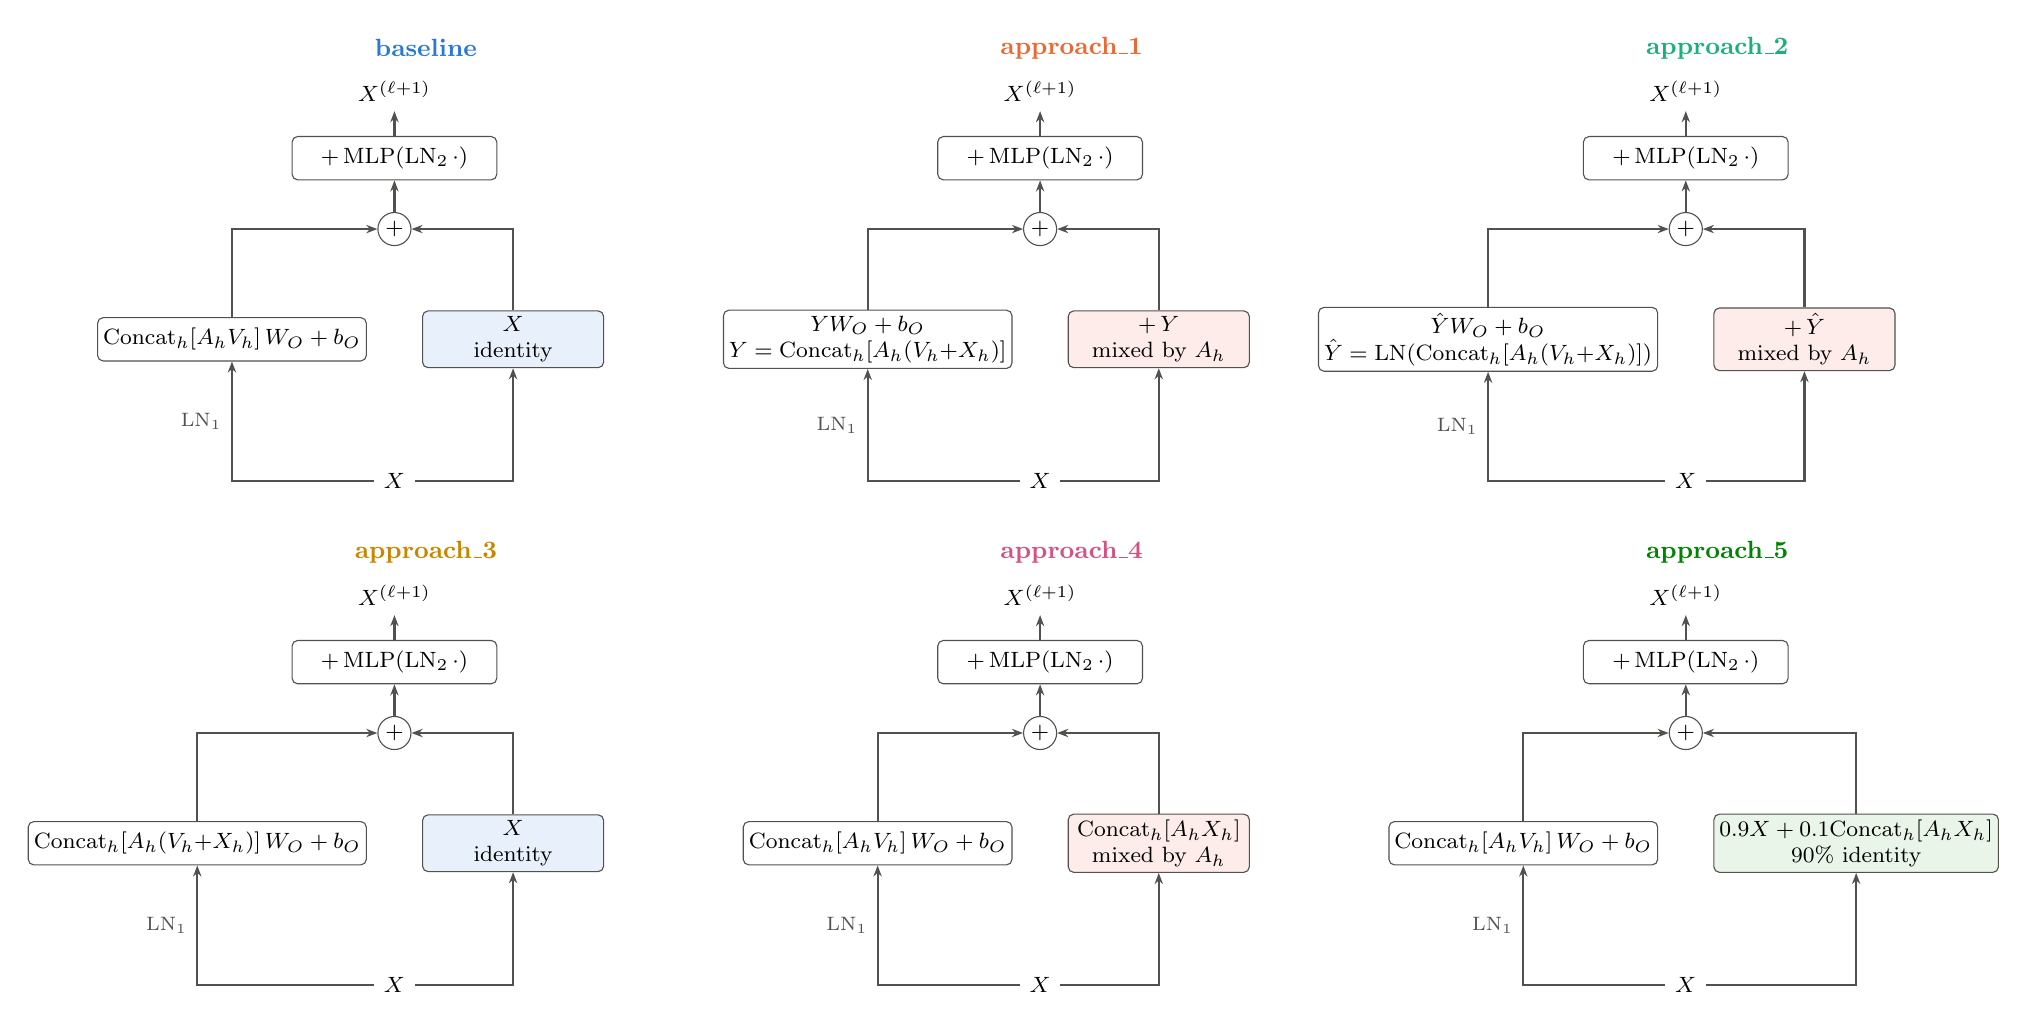
\begin{tikzpicture}[
  font=\footnotesize,
  box/.style={draw=ink2, rounded corners=2pt, minimum width=3.3cm, minimum height=0.55cm, align=center, fill=white, inner sep=2pt},
  sk/.style={draw=ink2, rounded corners=2pt, minimum width=2.3cm, minimum height=0.55cm, align=center, inner sep=2pt},
  op/.style={draw=ink2, circle, inner sep=0.5pt, minimum size=0.42cm, fill=white},
  arr/.style={-{Stealth[length=4pt]}, ink2, thick},
]
\newcommand{\panel}[7]{%
  % #1 x, #2 y, #3 title color, #4 title, #5 attention text, #6 skip text, #7 skip fill
  \begin{scope}[shift={(#1,#2)}]
    \node[font=\small\bfseries, text=#3] at (0.4,5.3) {#4};
    \node (xin) at (0,-0.2) {$X$};
    \node[box, anchor=east] (att) at (-0.35,1.6) {#5};
    \node[sk, fill=#7, anchor=west] (skip) at (0.35,1.6) {#6};
    \node[op] (add) at (0,3.0) {$+$};
    \node[box, minimum width=2.6cm] (mlp) at (0,3.9) {$+\,\mathrm{MLP}(\mathrm{LN}_2\,\cdot)$};
    \node (xout) at (0,4.75) {$X^{(\ell+1)}$};
    \draw[arr] (xin) -| node[pos=0.75, left, font=\scriptsize] {$\mathrm{LN}_1$} (att.south);
    \draw[arr] (xin) -| (skip.south);
    \draw[arr] (att.north) |- (add.west);
    \draw[arr] (skip.north) |- (add.east);
    \draw[arr] (add) -- (mlp); \draw[arr] (mlp) -- (xout);
  \end{scope}}
\panel{0}{6.4}{cbase}{baseline}{$\cat[A_hV_h]\,W_O + b_O$}{$X$\\identity}{okfill}
\panel{8.2}{6.4}{cone}{approach\_1}{$Y W_O + b_O$\\$Y=\cat[A_h(V_h{+}X_h)]$}{$+\,Y$\\mixed by $A_h$}{badfill}
\panel{16.4}{6.4}{ctwo}{approach\_2}{$\hat Y W_O + b_O$\\$\hat Y=\mathrm{LN}(\cat[A_h(V_h{+}X_h)])$}{$+\,\hat Y$\\mixed by $A_h$}{badfill}
\panel{0}{0}{cthree}{approach\_3}{$\cat[A_h(V_h{+}X_h)]\,W_O + b_O$}{$X$\\identity}{okfill}
\panel{8.2}{0}{cfour}{approach\_4}{$\cat[A_hV_h]\,W_O + b_O$}{$\cat[A_hX_h]$\\mixed by $A_h$}{badfill}
\panel{16.4}{0}{cfive}{approach\_5}{$\cat[A_hV_h]\,W_O + b_O$}{$0.9X + 0.1\cat[A_hX_h]$\\90\% identity}{midfill}
\end{tikzpicture}}
\caption{Each variant as an attention term (left) plus a skip path (right) that carries the token's own
state. Skip-path fill: blue, an identity path ($x_i$ passes unchanged); red, the state reaches the next layer
only after averaging by $A_h$; green, a 90/10 blend. In approach\_1 and 2, $Y$ also feeds the attention term,
so the box shows only the part that bypasses $W_O$. Red skip paths collapsed in training; blue and green
trained.}
\label{fig:arch}
\end{figure}

\section{Performance}
\begin{figure}[H]
\centering
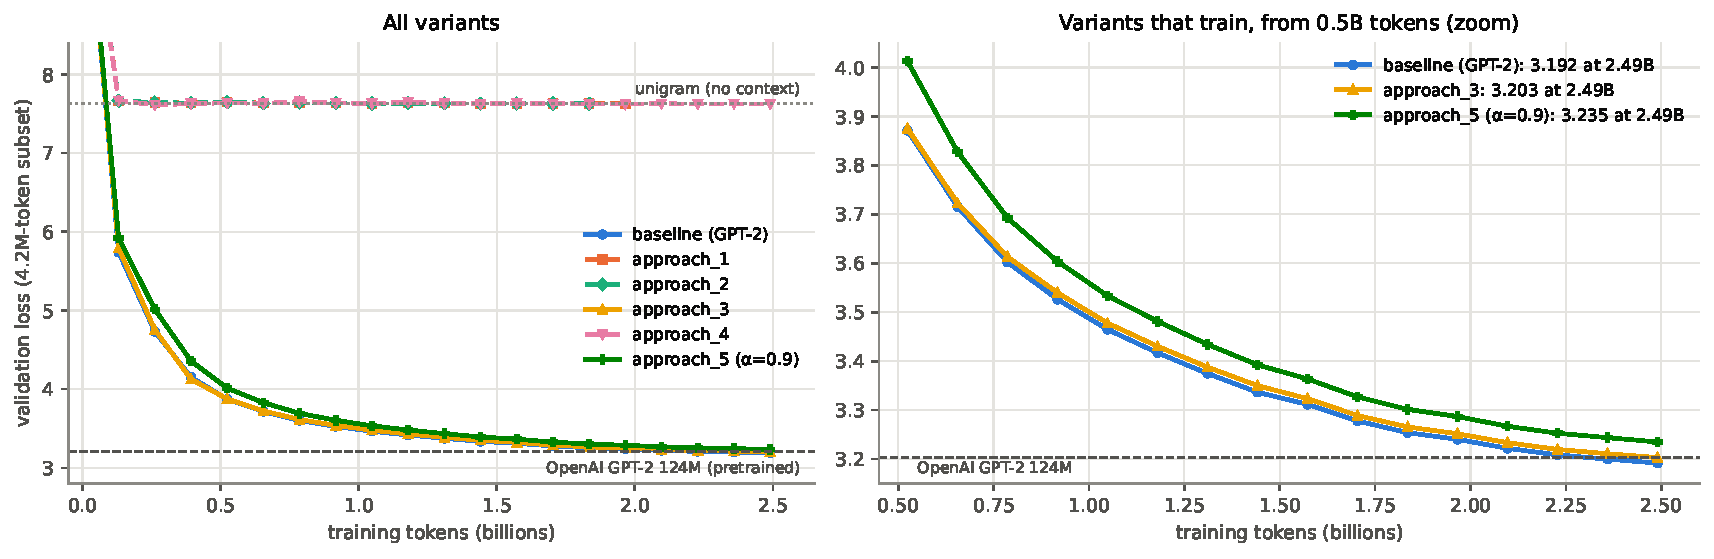
\includegraphics[width=\linewidth]{figures/fig_val_loss.pdf}
\caption{Validation loss (4.2M-token subset) every 250 steps. Left: every variant either follows the
baseline or drops to the unigram line within 250 steps and stays there. Right: zoom on the three that train.
The dashed line is the pretrained GPT-2 on the same 4.2M tokens (\RefFour).}
\label{fig:val}
\end{figure}

\begin{center}\small
\begin{tabular}{lrrrrrrl}
\toprule
& \multicolumn{5}{c}{Val loss at step (4.2M subset)} & Final & \\
Model & 250 & 500 & 1000 & 2000 & 3000 & 20M split & \\
\midrule
baseline   & \BaseAtA & \BaseAtB & \BaseAtC & \BaseAtD & \BaseAtE & \BaseTwenty & \\
approach\_3 & \ThreeAtA & \ThreeAtB & \ThreeAtC & \ThreeAtD & \ThreeAtE & \ThreeTwenty & \\
approach\_5 & \FiveAtA & \FiveAtB & \FiveAtC & \FiveAtD & \FiveAtE & \FiveTwenty & \\
approach\_1 & \OneAtA & \OneAtB & \OneAtC & \OneAtD & \OneAtE & \OneTwenty & \\
approach\_2 & \TwoAtA & \TwoAtB & \TwoAtC & \TwoAtD & \TwoAtE & \TwoTwenty & \\
approach\_4 & \FourAtA & \FourAtB & \FourAtC & \FourAtD & \FourAtE & \FourTwenty & \\
\bottomrule
\end{tabular}
\end{center}

\textbf{approach\_4 over the full run.} The first approach\_4 run was stopped at step 270. It was rerun for all
4768 steps to check that the collapse is permanent. From step 250 to the end, its validation loss stays between
7.61 and 7.67 with no downward trend. Its final loss on the 20M split, \FourTwenty, equals the unigram model's
\UniTwenty. Its gradients differ from approach\_1/2's. After step 400 the pre-clip gradient norm is large and
erratic: median 2.1, 90th percentile 15 (approach\_1: 0.14; baseline: 0.3; Figure~\ref{fig:train}). Clipping
caps each update at norm 1.0, and the loss does not move in response.

\begin{figure}[H]
\centering
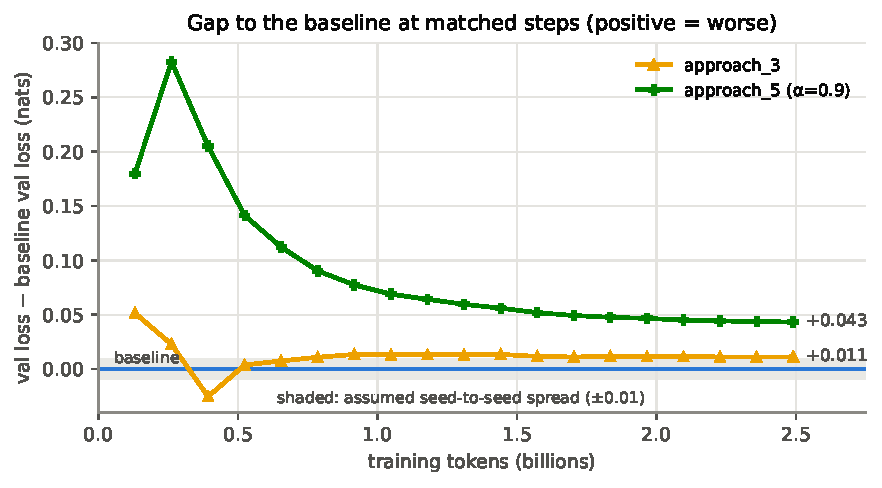
\includegraphics[width=0.78\linewidth]{figures/fig_gap_to_baseline.pdf}
\caption{Validation-loss gap to the baseline at the same step. approach\_3 settles at about $+0.011$ from
1B tokens on, which is about the size of seed-to-seed variation. approach\_5 starts far behind (peak $+0.28$ at
step 500), closes quickly until about 1B tokens, then flattens at $+0.043$.}
\label{fig:gap}
\end{figure}

\begin{figure}[H]
\centering
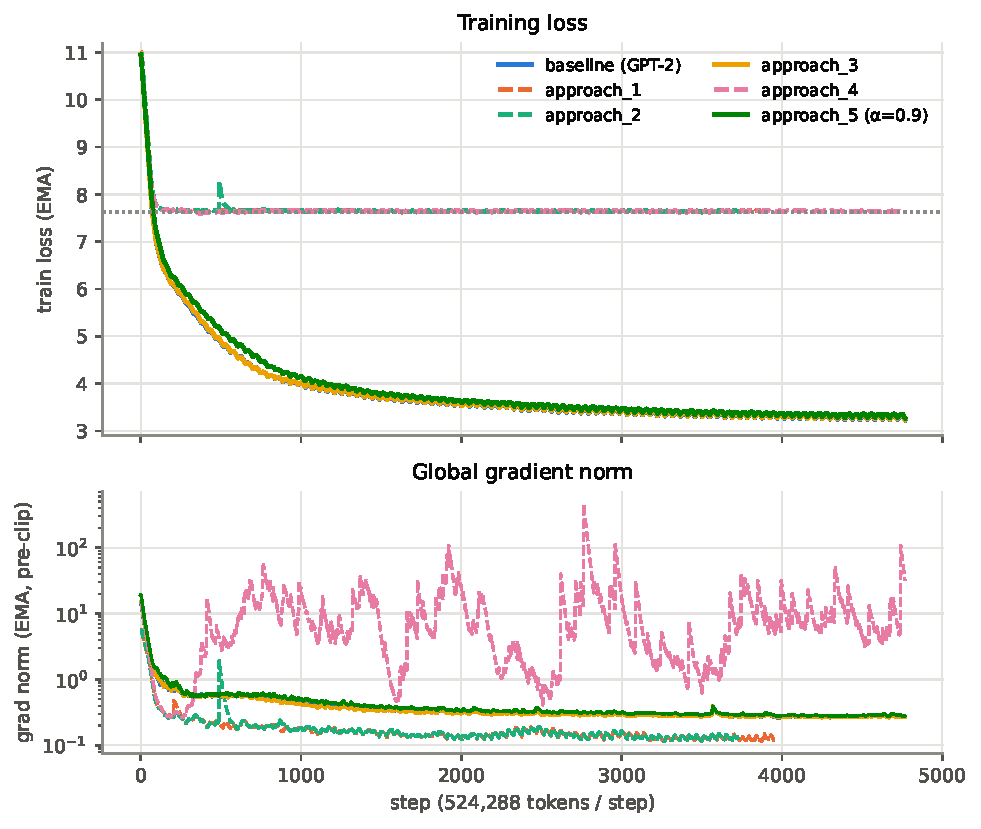
\includegraphics[width=0.72\linewidth]{figures/fig_train_dynamics.pdf}
\caption{Training loss and gradient norm. The collapsed variants (dashed) reach the unigram plateau by step
$\sim$150, and their gradient norm settles $2$--$3\times$ below the trained models'. approach\_2's spike at step
489 (loss 20.3) returns to the same plateau within about 10 steps.}
\label{fig:train}
\end{figure}

\paragraph{Reading the results.}
\begin{itemize}
\item \textbf{Three variants collapse.} approach\_1, 2 and 4 match the unigram model to within 0.004 nats
(\OneTwenty, \TwoTwenty{} vs.\ \UniTwenty) and their predictions are identical at every position (Section~\ref{sec:collapse}).
\item \textbf{approach\_3 ties the baseline.} Its gap of \ThreeDelta{} is consistent across 14 checkpoints
but is about the size of seed noise for runs this size (only one seed per variant was run).
\item \textbf{approach\_5 is clearly worse} by \FiveDelta, about 4$\times$ that noise level. The gap shrinks
by only $\sim$0.001 per 0.13B tokens at the end, so it would not close within this budget.
\item The baseline ends level with OpenAI's pretrained GPT-2 (\BaseTwenty{} vs.\ \RefTwenty), which confirms the
training pipeline. GPT-2 is scored off its training distribution, so this is context only.
\end{itemize}

\section{Why some variants work and others do not}
\subsection{Averaging the skip path causes rank collapse, already at initialization}\label{sec:collapse}
At initialization $Q,K$ are small, so $A_h\approx P$ with $P_{ij}=\frac{1}{i+1}[j\le i]$. If the skip path is
$\cat[A_hX_h]\approx PX$, every layer replaces each token's state with the mean of its prefix. $P$ is
row-stochastic and its only fixed direction is the constant vector, so repeated application drives every
position toward the same vector: the residual stream becomes rank 1. approach\_5 applies
$\alpha I + (1-\alpha)P$ instead, which keeps a fraction $\alpha$ of each token's own state per layer. The
attention and MLP outputs add further (partly averaged) content on top in every variant.

We measured this directly on the randomly initialized 12-layer models. \emph{Distance from rank 1} is
$\|X-\mathbf 1\bar x^\top\|_F/\|X\|_F$: 1 for unrelated positions, 0 when every position holds the same vector.

\begin{figure}[H]
\centering
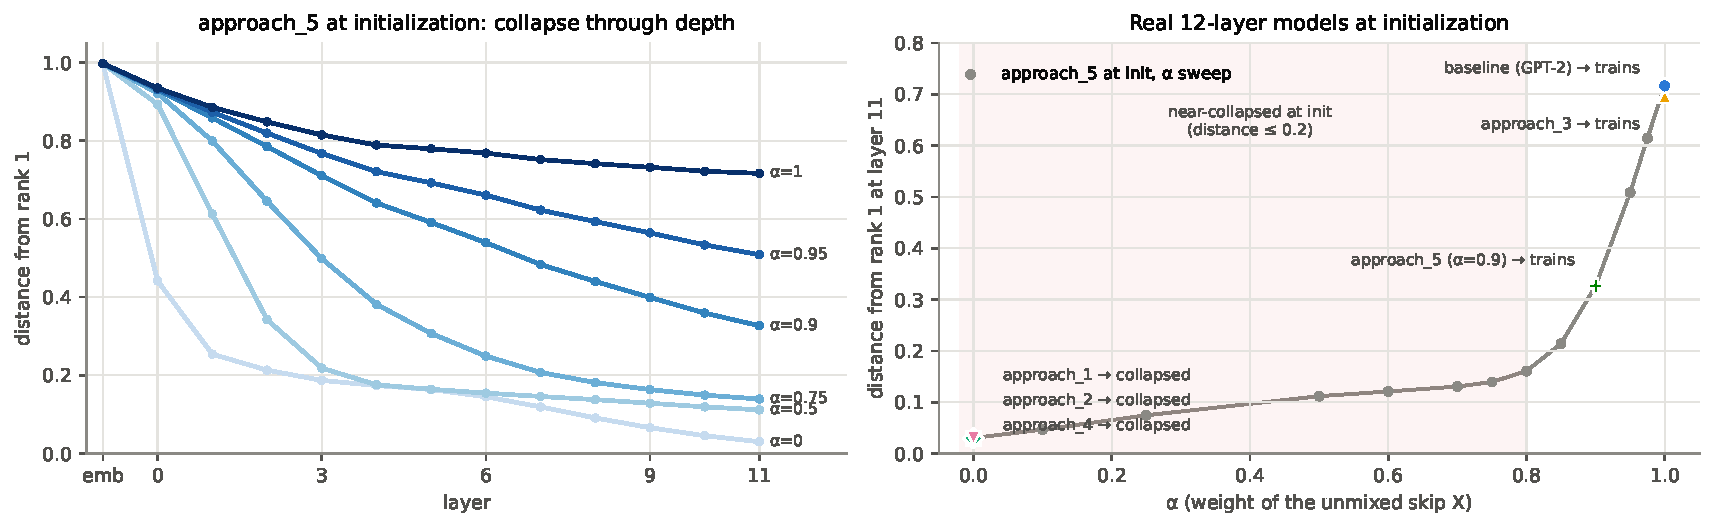
\includegraphics[width=\linewidth]{figures/fig_alpha_and_collapse.pdf}
\caption{Left: distance from rank 1 through depth for approach\_5 at initialization, for several $\alpha$
($\alpha{=}0$ is approach\_4; $\alpha{=}1$ is the baseline's identity skip plus approach\_4's attention term).
Right: the layer-11 value against $\alpha$, with every variant's initialization marked and its training outcome
annotated. Every variant at or below about 0.15 collapsed in training; every variant at 0.33 or above trained.}
\label{fig:alpha}
\end{figure}

\begin{center}\small
\begin{tabular}{lrrrl}
\toprule
& \multicolumn{2}{c}{At initialization (layer 11)} & Trained (layer 11) & \\
Model & distance from rank 1 & cosine between positions & distance from rank 1 & Outcome \\
\midrule
baseline   & \BaseInitRank & \BaseInitCos & \BaseTrRank & trains \\
approach\_3 & \ThreeInitRank & \ThreeInitCos & \ThreeTrRank & trains \\
approach\_5 & \FiveInitRank & \FiveInitCos & \FiveTrRank & trains (recovers) \\
approach\_1 & \OneInitRank & \OneInitCos & \OneTrRank & collapsed \\
approach\_2 & \TwoInitRank & \TwoInitCos & \TwoTrRank & collapsed \\
approach\_4 & \FourInitRank & \FourInitCos & \FourTrRank & collapsed \\
\bottomrule
\end{tabular}
\end{center}

This initialization probe takes seconds and correctly predicted the outcome of all six runs before
training. approach\_4's collapse was predicted from it and then confirmed over the full 2.5B tokens.

\subsection{Once collapsed, attention cannot learn: a zero-gradient fixed point}
\begin{prop}
If a layer's input is identical at every position, $X=\mathbf 1x^\top$, then that layer's attention is
uniform and the loss gradient with respect to its attention logits is exactly zero.
\end{prop}
\begin{proof}
$\mathrm{LN}_1$ is per-position, so all $q_i$, $k_j$, $v_j$ and $x_{h,j}$ are equal. The logits
$S_{ij}=q\cdot k/\sqrt{d_h}$ are constant over the causal prefix, so $A$ is uniform. With $u_j=v_j+x_{h,j}=u$
(or $u_j = v_j$, or $u_j = x_{h,j}$) and $g_i=\partial\mathcal L/\partial O_i$, the softmax Jacobian gives
$\partial\mathcal L/\partial S_{ij}=A_{ij}\big(g_i\cdot u_j-\sum_k A_{ik}\,g_i\cdot u_k\big)=0$.
\end{proof}
At initialization, the collapsed variants' streams are within 3\% of rank 1 by layer 11 and within 26\% after
layer 1, so the upper layers get almost no signal to sharpen their attention. Fitting token frequencies needs only
a constant output, so the optimizer finds it easier to collapse \emph{further}: the layer-11 distance falls from
0.03 to $\le$0.002, and the per-position KL to the unigram distribution is \OneKL, \TwoKL{} and \FourKL{}
(approach\_1, 2, 4). In approach\_1/2, the attention in every layer above 0 is exactly uniform
(Figures~\ref{fig:layers} and \ref{fig:heat}).

approach\_4 reaches the same end state by a different route. Its trained attention is \emph{sharp}, not
uniform: in layers 0--2 the largest weight per query averages 0.85--0.94. But within a head, most queries
choose the same source position: 28\%, 47\% and 83\% of queries in layers 0, 1 and 2, measured on 4 validation
sequences, positions $\ge 64$. In layers 5 and 11 every query attends to the same few early tokens (the
vertical stripes in Figure~\ref{fig:heat}). Since its skip path is $\cat[A_hX_h]$, every token then copies
the same $X_h$. The positions become identical (cosine 1.000 from layer 4 on; layer-11 distance from rank 1
\FourTrRank), and the output is again the unigram distribution. Sharp attention to a \emph{shared} source
collapses the stream just as uniform attention does. Only an unmixed path for each token's own state prevents
it.

approach\_5 starts partly collapsed (0.33), but not at the fixed point. Its gradients are small but nonzero, so the
heads can sharpen. They do: by the end of training the stream's distance from rank 1 is \FiveTrRank, the same as the
baseline's \BaseTrRank. The slow start is visible as the gap's peak of $+0.28$ at step 500 (Figure~\ref{fig:gap}).

\begin{figure}[H]
\centering
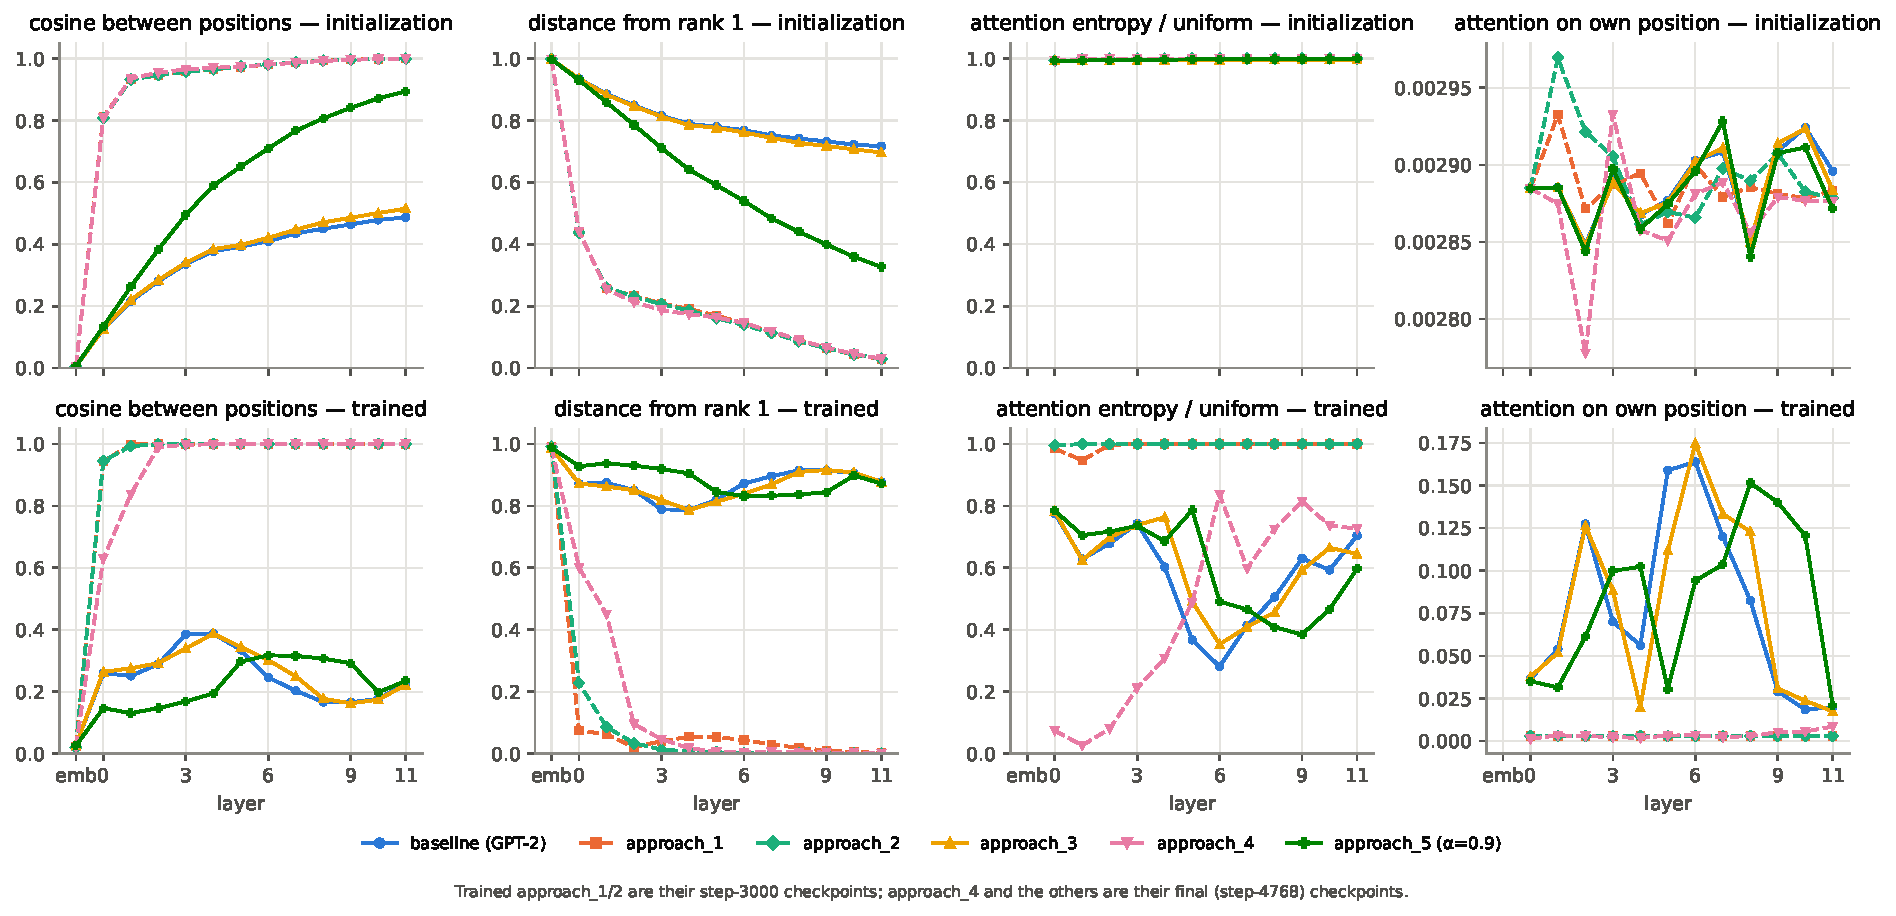
\includegraphics[width=\linewidth]{figures/fig_layer_diagnostics.pdf}
\caption{Per-layer diagnostics on 8 validation sequences (positions $\ge 64$). Top row: initialization.
Bottom row: trained. All three collapsed variants (dashed) end with identical positions (cosine 1) and
near-zero self-weight. approach\_1/2 do so with uniform attention (entropy ratio 1); approach\_4 does so with
sharper attention (entropy ratio 0.03--0.8) aimed at shared positions. approach\_5 starts between the two groups and ends with the
trained ones.}
\label{fig:layers}
\end{figure}

\begin{figure}[H]
\centering
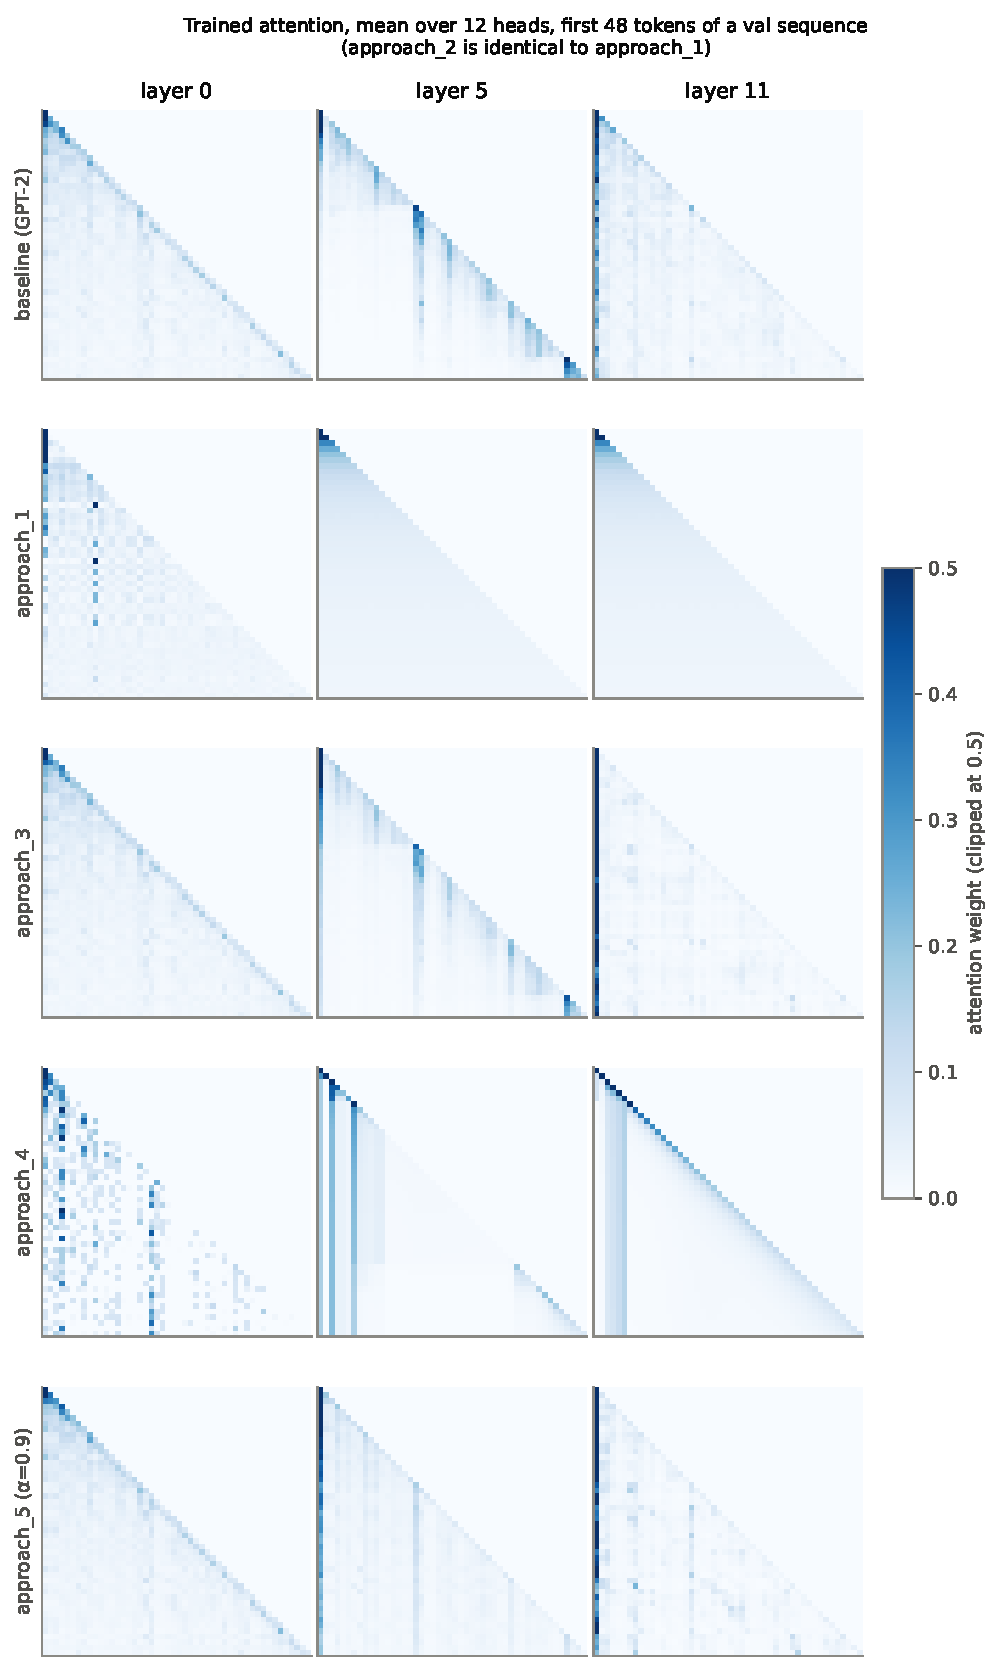
\includegraphics[width=0.66\linewidth]{figures/fig_attention_heatmaps.pdf}
\caption{Trained attention, mean over heads. approach\_1's layers 5 and 11 are exactly uniform over the prefix
(row $i$ is $1/(i{+}1)$). The baseline and approach\_3 have nearly identical patterns. approach\_5 has less of the
baseline's local and diagonal structure at layer 5, and more attention on the first token. approach\_4
(full run) is sharp but shared: in layers 5 and 11, every query attends to the same few early positions
(vertical stripes).}
\label{fig:heat}
\end{figure}

\subsection{Why approach\_5 trains but costs \FiveDelta{} nats}
Three properties of $\alpha X + (1-\alpha)\cat[A_hX_h]$ make it strictly harder than the identity skip:
\begin{enumerate}
\item \textbf{Earlier layers fade.} The skip path scales the stream by $\alpha$ per layer, so whatever layer
$\ell$ writes reaches the top attenuated by $\alpha^{11-\ell}$: $0.9^{11}\approx 0.31$ for layer 0. The baseline
keeps it at full strength. In the trained model, the residual norm stays near 22 from layer 5 to layer 10, while
the baseline's grows to 37 (Figure~\ref{fig:mech}, right). Information that must survive to the top has to be
re-written by later layers.
\item \textbf{One attention matrix, two jobs.} $A_h$ both reads context (through $V_h$) and decides what is
blended into the token's own state (through $X_h$). A head that attends far away for $V_h$ also blurs
$X_h$ by 10\%. The trained approach\_5 moves self-attention to layers 8--10 (weight 0.12--0.15 vs.\ 0.02--0.08 in the
baseline, Figure~\ref{fig:mech}, middle). This is consistent with heads limiting the blur, but the summed
self-weight over all layers is similar (0.99 vs.\ 0.94), so it is a reallocation, not a general increase.
\item \textbf{Slow start.} At initialization the stream is already partly collapsed (0.33 vs.\ 0.72), so the first
$\sim$500 steps make little use of context (Figure~\ref{fig:gap}).
\end{enumerate}

\begin{figure}[H]
\centering
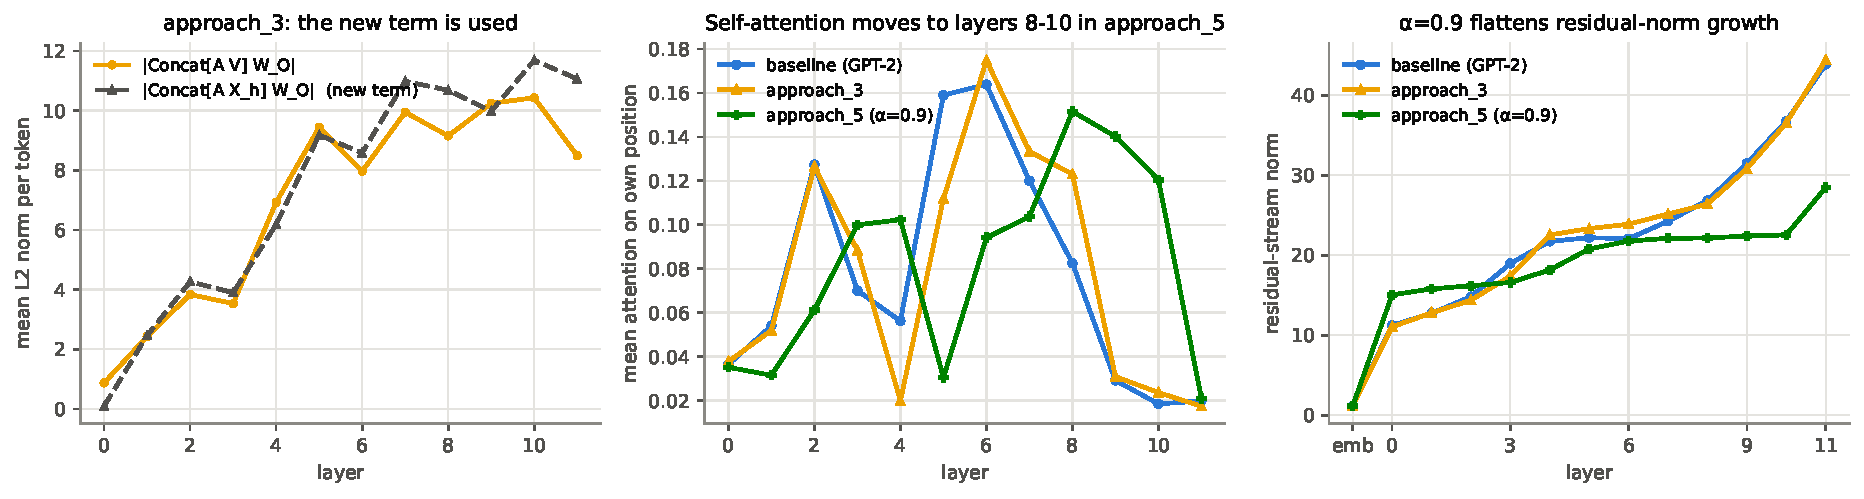
\includegraphics[width=\linewidth]{figures/fig_mechanism_trained.pdf}
\caption{Trained models. Left: in approach\_3, the new term $\cat[A_hX_h]W_O$ is as large as the standard attention
term in most layers. Middle: per-layer self-attention weight. Right: residual-stream norm through depth; with
$\alpha=0.9$ it stays near 22 from layer 5 to 10.}
\label{fig:mech}
\end{figure}

\subsection{Why approach\_3 ties the baseline but does not beat it}
approach\_3 keeps the identity skip, so it does not collapse. Its new term is used heavily. In most layers the
norm of $\cat[A_hX_h]W_O$ is about that of the standard term $\cat[A_hV_h]W_O$ (Figure~\ref{fig:mech}, left). But it adds little the model
could not already express. For head $h$,
\[
A_h(V_h + X_h)\,W_O^{(h)} = A_h\big(\mathrm{LN}_1(X)\,W_V^{(h)} + b_V^{(h)} + X E_h\big)\,W_O^{(h)},
\]
where $E_h$ selects the head's 64 coordinates. Both $V_h$ and $X_h$ are linear maps of the token state. They differ
only in that $V_h$ reads the per-token normalized state through a learned $W_V^{(h)}$, while $X_h$ reads the
unnormalized state through a fixed coordinate slice. The baseline can already learn $W_V^{(h)}\approx E_h$ up to
LayerNorm's per-token scale. So approach\_3 mainly changes the parametrization (a fixed, unnormalized extra
channel) rather than adding capability, which is consistent with the near-identical loss and attention patterns.

\section{Conclusions}
\begin{enumerate}
\item \textbf{Keep an unmixed path for each token's own state.} Every variant without one (approach\_1, 2, 4)
collapsed to the unigram model, at initialization and permanently. Normalizing (approach\_2) or moving
$W_O$ (approach\_4) does not change this.
\item \textbf{Partial mixing trains but costs quality.} approach\_5 with $\alpha=0.9$ recovers from a partly collapsed
start but ends \FiveDelta{} nats behind, mainly because the skip path is no longer an identity.
\item \textbf{Feeding $X_h$ into attention is harmless but not helpful} (approach\_3, \ThreeDelta, within noise).
$V_h$ is already a learned linear read of the same state.
\item \textbf{The initialization probe is a reliable, nearly free screen.} A layer-11 distance from rank 1 at or
below about 0.15 predicted collapse for every variant tested.
\end{enumerate}

\paragraph{Suggested next steps.}
(i) Make $\alpha$ a learnable per-layer scalar initialized at 1. If training keeps it near 1, that confirms mixing the
skip path does not help. (ii) Run 2--3 seeds of baseline and approach\_3 to establish whether \ThreeDelta{} is real
($\sim$35 min per run on 4 GPUs). (iii) Any new variant: run the initialization probe first.

\section*{Files}
{\small
\begin{tabularx}{\linewidth}{@{}lX@{}}
\code{report.tex}, \code{report.pdf}, \code{numbers.tex} & this report; all numbers are generated from the logs \\
\code{figures/} & all figures (PDF and PNG) \\
\code{data/<model>/log.jsonl}, \code{config.json} & per-step train loss, LR, grad norm, timing; val loss every 250 steps \\
\code{data/matched\_evals.json} & every model, the pretrained GPT-2 and the unigram on identical 4.2M and 20M val subsets \\
\code{data/variants\_probe.json} & per-layer diagnostics, initialization and trained \\
\code{data/alpha\_sweep.json} & approach\_5 initialization probe over $\alpha$ \\
\code{data/heatmaps.npz}, \code{data/summary.json} & attention maps; final numbers \\
\code{code/model.py}, \code{code/gpt2\_torch.py} & snapshot of \code{src/model.py} (code in Appendix~\ref{app:code}) and the trained PyTorch port \\
\end{tabularx}}

{\raggedright Regenerate with \code{train/analyze\_variants.py} (GPU diagnostics and matched evals) and
\code{train/make\_variant\_report.py} (figures and numbers), then \code{pdflatex report.tex}. Checkpoints are in
\code{runs/chinchilla/} under \code{/local/scratch/a/liu3170}.\par}

\clearpage
\appendix
\sloppy
\section{Code for each variant (from \code{src/model.py})}\label{app:code}

All listings are taken verbatim from \code{src/model.py}, including comments. A snapshot of the file is saved in
\code{code/model.py}. Line numbers are the file's own. For each variant, only the lines of \code{attn} and
\code{block} that run for its \code{hparams} setting are shown. A jump in the line numbers means the lines in
between belong to other variants or to the \code{past} (incremental decoding) path. The training runs used the
PyTorch port \code{train/gpt2\_torch.py} (snapshot in \code{code/gpt2\_torch.py}), which implements the same
equations.

\lstset{numbers=left, numberstyle=\tiny\color{ink2}, numbersep=6pt, xleftmargin=18pt, consecutivenumbers=false}
\newcommand{\varcode}[5]{\subsection{#1}\noindent{\small #2\\\code{#3}}\par\nopagebreak
\lstinputlisting[linerange={#4}, title={in \code{attn()}}]{code/model.py}
\lstinputlisting[linerange={#5}, title={in \code{block()}}]{code/model.py}}

\subsection{Shared code}
The settings (\code{default\_hparams}), the LayerNorm with the \code{affine} switch that approach\_2 uses, and
the per-head attention \code{multihead\_attn}. Its \code{x\_heads} argument adds $X_h$ to $V_h$ before
$A_h$ is applied.
\lstinputlisting[linerange={18-33}, title={\code{default\_hparams()}}]{code/model.py}
\lstinputlisting[linerange={49-61}, title={\code{norm()}}]{code/model.py}
\lstinputlisting[linerange={114-125}, title={\code{multihead\_attn()}, inside \code{attn()}}]{code/model.py}

\varcode{Baseline (original GPT-2)}{$X' = X + \cat[A_hV_h]\,W_O + b_O$.}
{attn\_residual=False, attn\_proj\_residual=None}
{128-130,135-135,140-141,151-152,155-156,159-159}{173-174,176-180}

\varcode{approach\_1}{$Y=\cat[A_h(V_h+X_h)]$,\quad $X' = YW_O + b_O + Y$.}
{attn\_residual=True, attn\_proj\_residual='approach\_1'}
{128-130,135-135,139-139,151-152,155-159}{173-175,178-180}

\varcode{approach\_2}{$Y=\mathrm{LN}(\cat[A_h(V_h+X_h)])$ (no affine),\quad $X' = YW_O + b_O + Y$.}
{attn\_residual=True, attn\_proj\_residual='approach\_2'}
{128-130,135-135,139-139,151-159}{173-175,178-180}

\varcode{approach\_3}{$Y=\cat[A_h(V_h+X_h)]$,\quad $X' = X + YW_O + b_O$.}
{attn\_residual=True, attn\_proj\_residual='approach\_3'}
{128-130,135-135,139-139,151-152,155-156,159-159}{173-174,176-180}

\varcode{approach\_4}{$X' = \cat[A_hV_h]\,W_O + b_O + \cat[A_hX_h]$.}
{attn\_residual=True, attn\_proj\_residual='approach\_4'}
{128-130,135-135,139-139,143-143,145-146,149-150}{173-175,178-180}

\varcode{approach\_5}{$X' = \cat[A_hV_h]\,W_O + b_O + \alpha X + (1-\alpha)\cat[A_hX_h]$, $\alpha=0.9$.}
{attn\_residual=True, attn\_proj\_residual='approach\_5', attn\_alpha=0.9}
{128-130,135-135,139-139,143-143,145-150}{173-175,178-180}

\subsection{Complete \code{attn} and \code{block}}\label{app:full}
The full functions, unedited, with all branches.
\lstinputlisting[firstline=92, lastline=180]{code/model.py}


\end{document}
